%%%%%%%%%%%%%%%%%%%%%%%%%%%%%%%%%%%%%%%%%%%%%%%%%%%%%%%%%%%%%%%%%
% Dissertacao de Mestrado / Dept Fisica, CFM, UFSC              %
% Andre@UFSC - 2011                                             %
%%%%%%%%%%%%%%%%%%%%%%%%%%%%%%%%%%%%%%%%%%%%%%%%%%%%%%%%%%%%%%%%%


%:::::::::::::::::::::::::::::::::::::::::::::::::::::::::::::::%
%                                                               %
%                          Capítulo 4                           %
%                                                               %
%:::::::::::::::::::::::::::::::::::::::::::::::::::::::::::::::%

%***************************************************************%
%                                                               %
%                    Problemas astrofísicos                     %
%                                                               %
%***************************************************************%

\chapter{Problemas astrofísicos}
\label{sec:Problemas}

Gaivota com cores UV.

Onde caem as diferentes classes (star forming, retired, passivas, AGN, etc, ver
ultimo paper do \citet{CidFernandes2011}) num diagrama parecido com o de
\citet{Chilingarian2011}. Revisar o artigo. 

(Retired != passivas) = legal!

\begin{figure}
	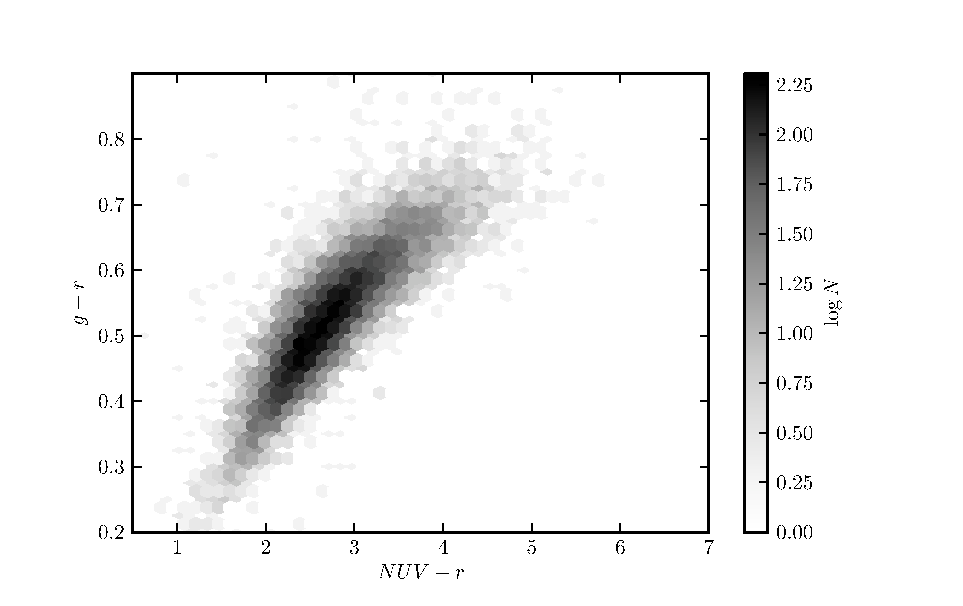
\includegraphics{figuras/uvcolor-color-density.eps}
	\caption[Densidade de galáxias no diagrama cor--cor UV.]
	{Densidade de galáxias em função de cor UV e cor óptica. Foram selecionados
	objetos da amostra do \starlight com $-23 > z > -21.5$. As magnitudes $g$, $r$
	e $z$ são do \SDSS. A intensidade dos bins corresponde ao logarítmo do número
	de objetos.}
	\label{fig:DensityColor}
\end{figure}

\begin{figure}
	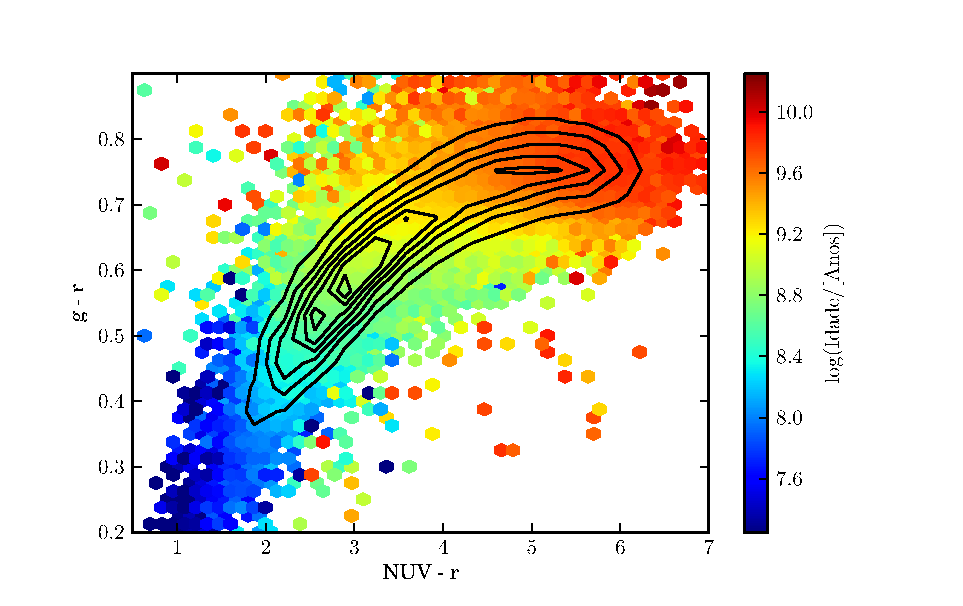
\includegraphics{figuras/uvcolor-color-at_flux.eps}
	\caption[Idade média das galáxias ponderada em fluxo no diagrama cor--cor UV.]
	{Idade média das galáxias ponderada em fluxo em função de cor UV e cor óptica.
	Os valores estão expressos em logarítmo da idade da galáxia em anos. O contorno
	indica a densidade de galáxias, conforme a figura \ref{fig:DensityColor}.}
	\label{fig:ATFluxColor}
\end{figure}

\begin{figure}
	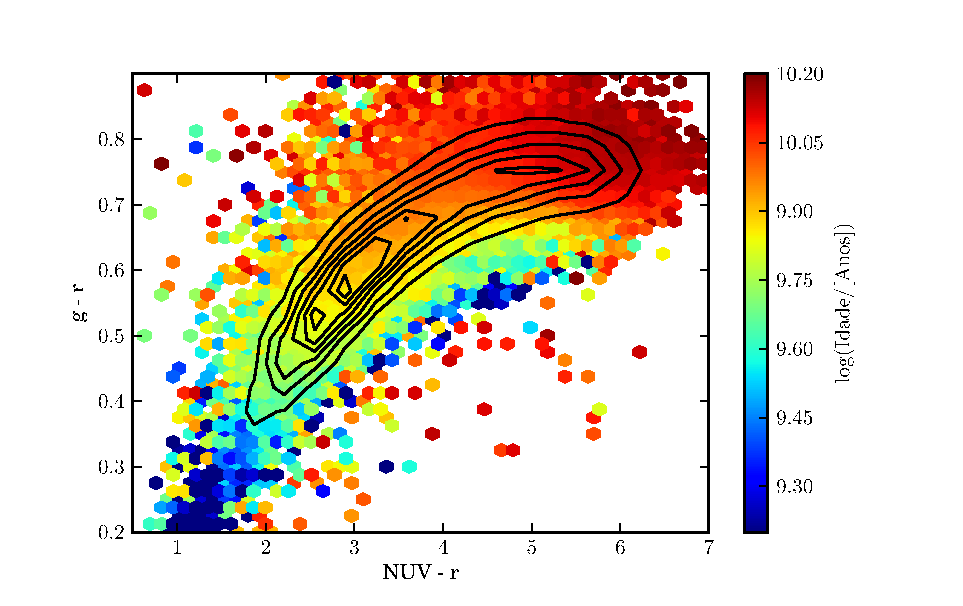
\includegraphics{figuras/uvcolor-color-at_mass.eps}
	\caption[Idade média das galáxias ponderada em massa no diagrama cor--cor UV.]
	{O mesmo que a figura \ref{fig:ATFluxColor}, para a idade ponderada em massa.
	Note que a escala de idades não é a mesma.}
	\label{fig:ATMassColor}
\end{figure}

\begin{figure}
	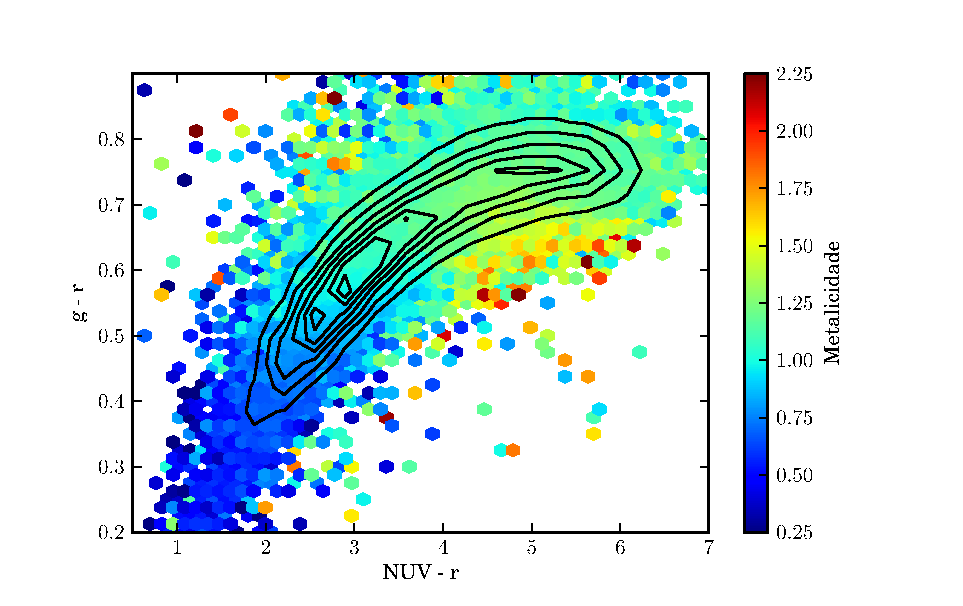
\includegraphics{figuras/uvcolor-color-am_flux.eps}
	\caption[Metalicidade das galáxias ponderada em fluxo no diagrama cor--cor UV.]
	{O mesmo que a figura \ref{fig:ATFluxColor}, para a metalicidade ponderada em
	fluxo.}
	\label{fig:AMFluxColor}
\end{figure}

\begin{figure}
	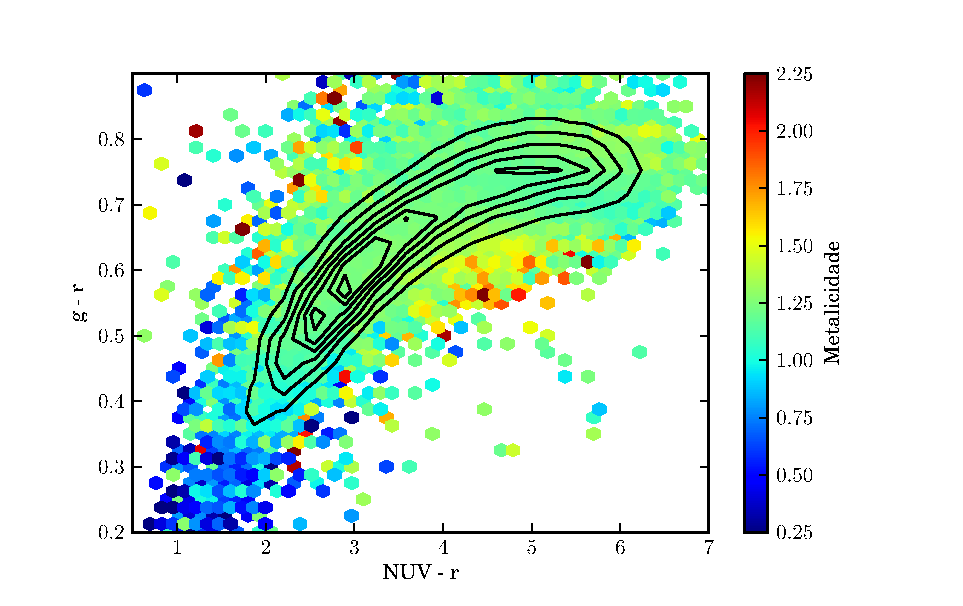
\includegraphics{figuras/uvcolor-color-am_mass.eps}
	\caption[Metalicidade das galáxias ponderada em massa no diagrama cor--cor UV.]
	{O mesmo que a figura \ref{fig:ATFluxColor}, para a metalicidade ponderada em
	massa.}
	\label{fig:AMMassColor}
\end{figure}

\begin{figure}
	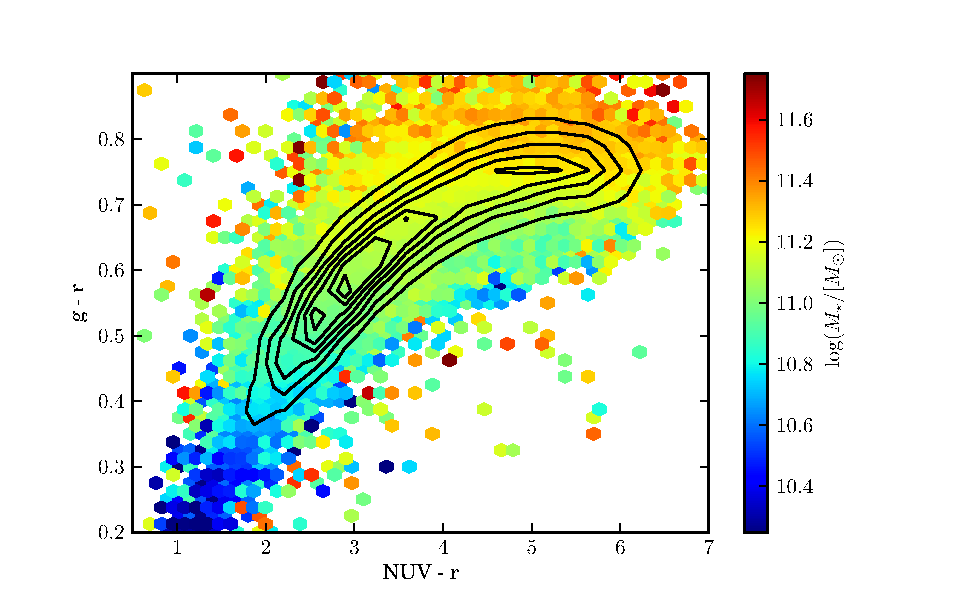
\includegraphics{figuras/uvcolor-color-mcor_gal.eps}
	\caption[Massa estelar das galáxias no diagrama cor--cor UV.]
	{O mesmo que a figura \ref{fig:ATFluxColor}, para a massa estelar das
	galáxias. Os valores são expressos como logarítmo da massa em massas solares.}
	\label{fig:MCorGalColor}
\end{figure}

\begin{figure}
	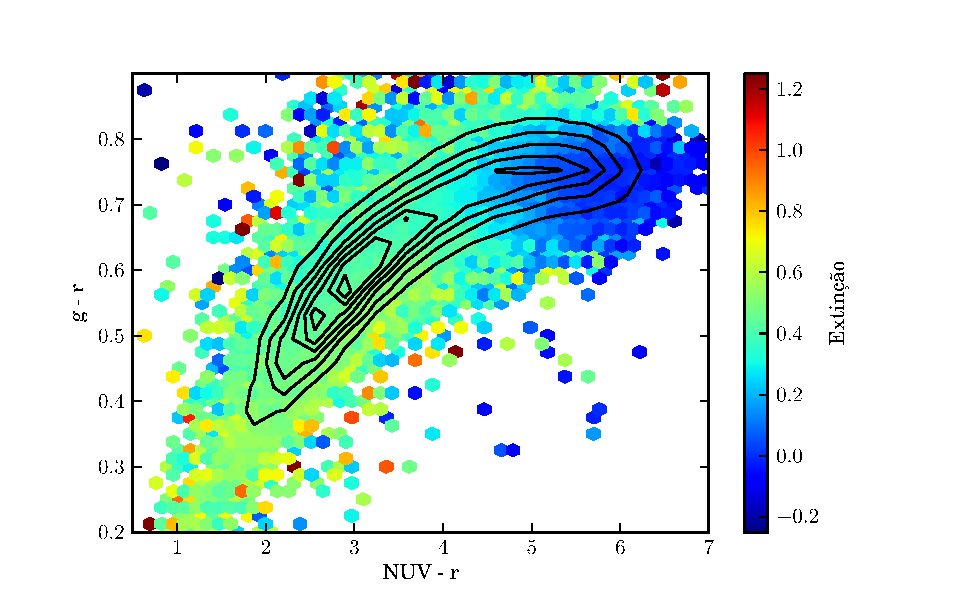
\includegraphics{figuras/uvcolor-color-AV.eps}
	\caption[Absorção por poeira no diagrama cor--cor UV.]
	{O mesmo que a figura \ref{fig:ATFluxColor}, para a extinção por
	poeira.}
	\label{fig:AV}
\end{figure}



% End of this chapter
